\section{Question 2}

\subsection{The Question}

\begin{flushleft}

Create a histogram of how many pages each blog has (e.g., 30
blogs with just one page, 27 with two pages, 29 with 3 pages and 
so on).

\end{flushleft}
\subsection{The Answer}



The expected outcome from intuition is that the histogram will follow a power-law trend where there are many blogs that contain few pages, at least one, but there are very few that have many pages. This result seems reasonable from previous assignments, but it is interesting if this simple ``many-few, few-many'' approach true characterizes the data, or is a useful approximation. 

\begin{wrapfigure}{r}{0.4\textwidth}
  \vspace{-20pt}
  \begin{center}
    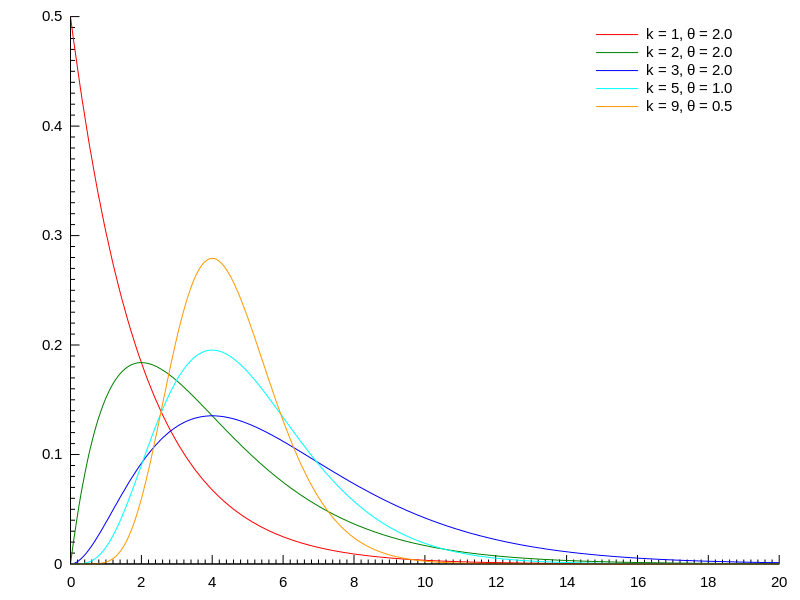
\includegraphics[width=0.4\textwidth]{gamma}
  \end{center}
  \vspace{-20pt}
  \caption{Gamma distributions}
  \vspace{-10pt}
\end{wrapfigure}



There is the possibility that there are very few bloggers that only have one page of feeds. Assuming someone was motivated to start blogging they would be very active in the beginning and write a substantial number of posts, enough for a few pages. Then the hype dies off and port become more infrequent and only the few committed bloggers stay active enough to collect many pages. But most people would write at least a few pages, meaning that the bulk of bloggers have some in between 1 or 2 pages and many pages. This is known as the Gamma distribution

The Gamma distribution describes a family of distributions, each with a different shape based on the parameter values. The known power-law distribution is a special case of the Gamma distribution. The Gamma distribution has the characteristic that it does not take negative values and is infinite in the positive direction. This is in contrast to the normal distribution that is defined for negative values. In this application a negative number of pages has no meaning and the Gamma distribution is the appropriate choice. Using the information from a useful blog post \cite{Rplots} we can create a histogram of the data and overlay the corresponding Gamma function fitted to the data's statistical modes, i.e. the mean and variance.


\lstset{
    language=R,
    label=code:q1,
    caption={R script to produce histogram and density plot}
}
\lstinputlisting{../q1/math.r}



\begin{figure}
\centering
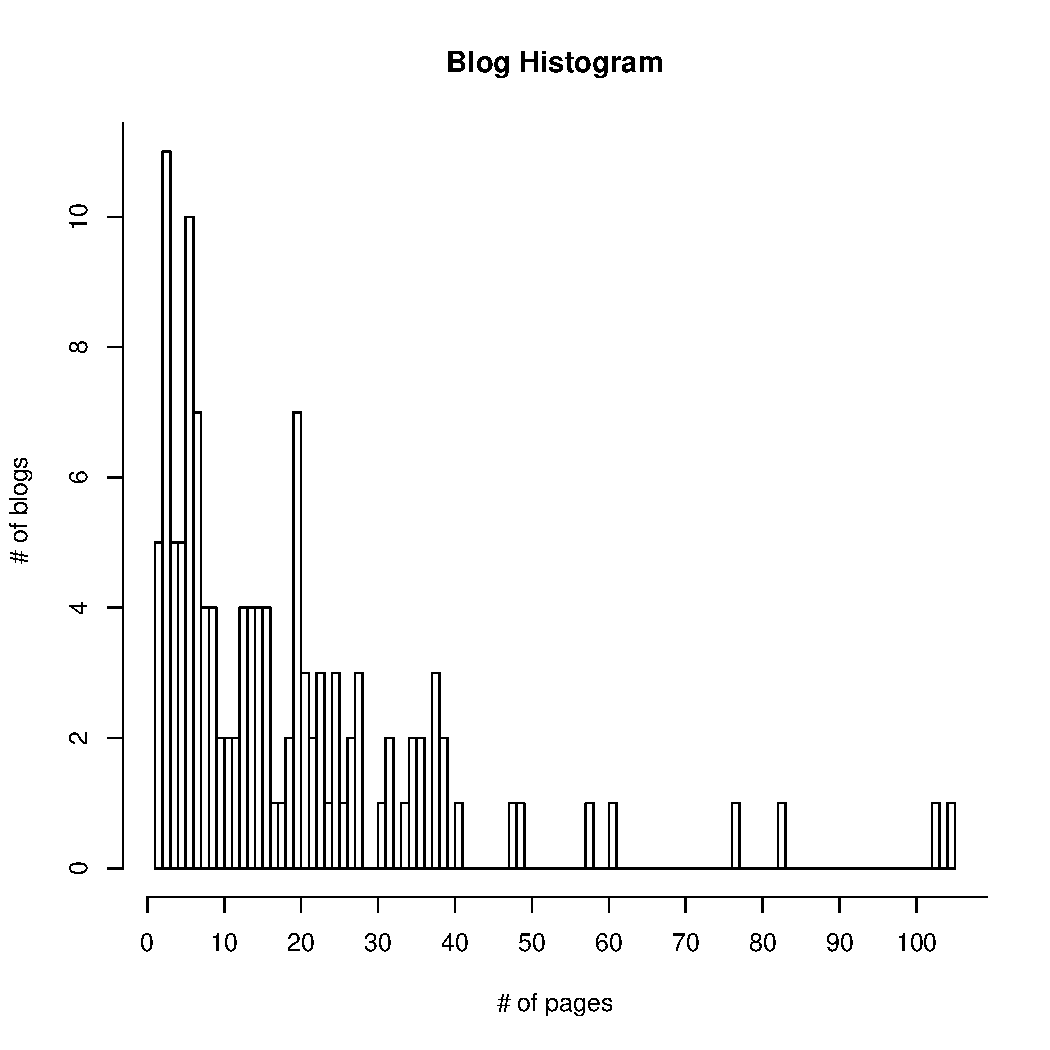
\includegraphics[width=.72\textwidth]{../q1/freqHist.pdf}

\end{figure}


\begin{figure}
\centering
\begin{subfigure}{.44\textwidth}
  \centering
  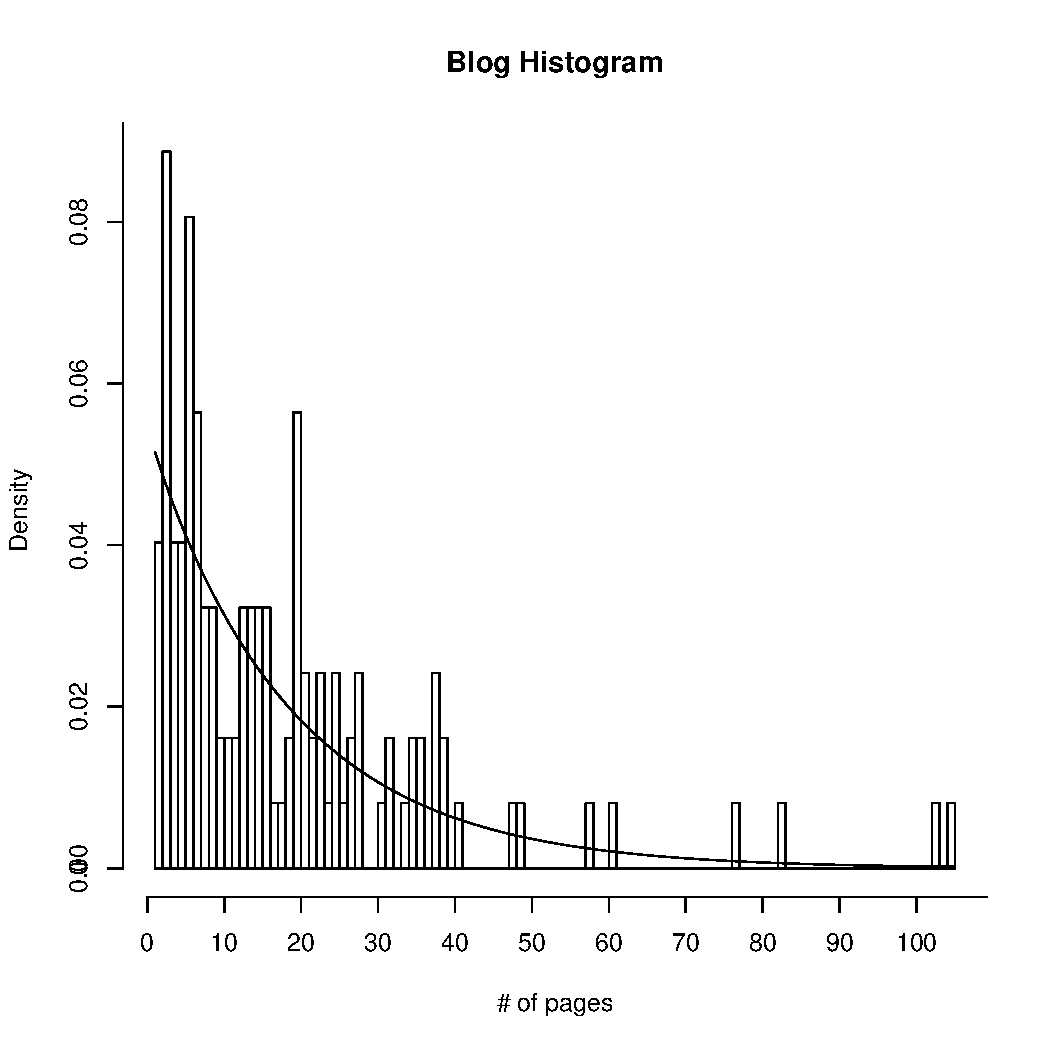
\includegraphics[width=\linewidth]{../q1/densHist.pdf}
  \caption{no. bins = no. blogs}

\end{subfigure}%
\begin{subfigure}{.44\textwidth}
  \centering
  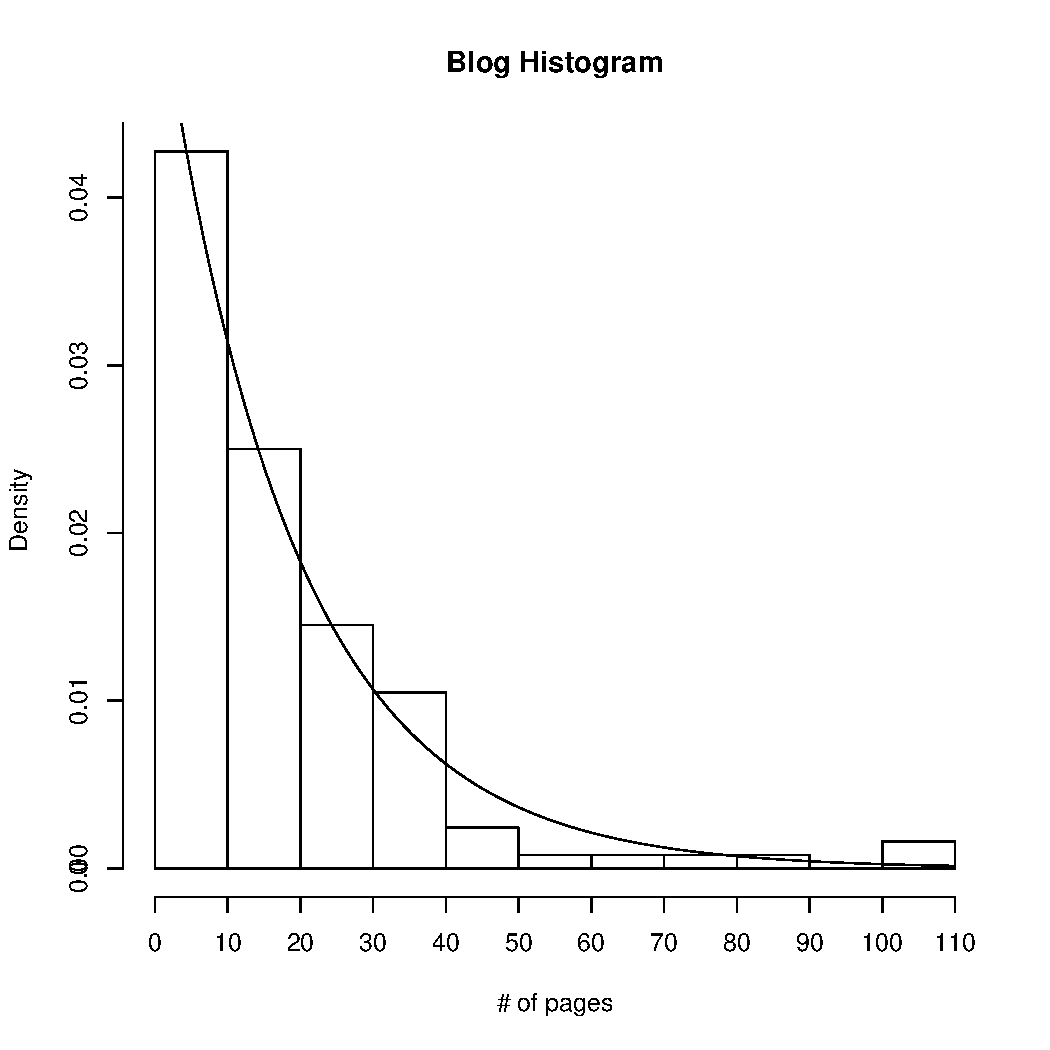
\includegraphics[width=\linewidth]{../q1/densHist1.pdf}
  \caption{no. bins = 10 (default)}

\end{subfigure}
\caption{Density Histogram with fitted Gamma distribution}
\label{fig:test}
\end{figure}
